\sectioncounter{35}

\section{平面与平面的垂直}

\subsection{知识梳理}

设半平面 $\alpha$,$\beta$ 有公共棱 $l$, 则该图形记为二面角 $\alpha\text{--}l\text{--}\beta$, 叫做 $\alpha$ 与 $\beta$ 所成的二面角. 任取 $l$ 上一点 $P$, 在 $\alpha$ 内作 $PA\perp l$ 于点 $P$, 在 $\beta$ 内作 $PB\perp l$ 于点 $P$, 则 $\angle APB$ 称为二面角 $\alpha\text{--}l\text{--}\beta$ 的平面角, 其大小称为该二面角的大小. 若在 $l$ 上再任取一点 $Q$, 则此时二面角 $\alpha\text{--}l\text{--}\beta$ 也可记为二面角 $A\text{--}PQ\text{--}B$.

若两个相交平面所成二面角是直二面角, 则称这两个平面互相垂直. 除了定义以外, 还可用下述定理判定两个平面垂直.

面面垂直判定定理: 一个平面过另一个平面的垂线, 则这两个平面互相垂直.

对应的符号语言 (图 \ref{fig-190703-1930}): $l\perp\alpha$, $l\subset\beta$ $\Rightarrow$ $\alpha\perp\beta$.

面面垂直性质定理: 两个平面垂直, 则一个平面内垂直于交线的直线与另一个平面垂直.

对应的符号语言 (图 \ref{fig-190703-1940}): $\alpha\perp\beta$, $\alpha\cap\beta= AB$, $CD\subset\beta$ 且 $CD\perp AB$ 于点 $D$ $\Rightarrow$ $CD\perp\alpha$.

面面垂直性质定理的推论: 两个平面垂直, 过一个平面内一点作另一个面的垂线, 则垂线在前一个平面内.

对应的符号语言 (如图 \ref{fig-190703-1940}): $\alpha\perp\beta$, $C\in\beta$, $CD\perp\alpha$ $\Rightarrow$ $CD\subset\beta$.
 
    \begin{figure}[htb]
    \small
    \centering
    \begin{minipage}[b]{0.45\linewidth}
      \centering
      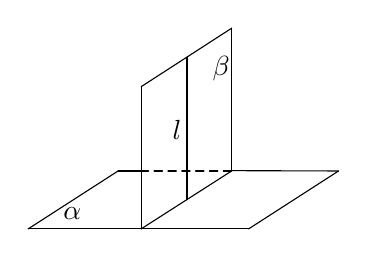
\begin{tikzpicture}[line cap=round,line join=round,scale=0.7]        
        \draw (0,0)-- (1.63,1.05);
        \draw (5.63,1.05)-- (4,0);
        \draw (2.05,2.58)-- (3.69,3.64);
        \draw (0,0)-- (4,0);
        \draw (2.05,2.583)-- (2.05,0);
        \draw (2.05,0)-- (3.69,1.05);
        \draw (3.69,1.05)-- (3.69,3.64);
        \draw (2.88,3.11)-- (2.88,0.53);
        \draw (1.63,1.05)-- (2.05,1.05);
        \draw [densely dashed] (3.69,1.05)-- (2.05,1.05);
        \draw (3.69,1.056)-- (5.63,1.05);

        \draw (0.8,0) node[above] {$\alpha$};
        \draw (3.5,2.9) node {$\beta$};
        \draw (2.7,1.8) node {$l$};  
      \end{tikzpicture}
      \caption{}\label{fig-190703-1930}
    \end{minipage}
    \hskip 0.5cm  
    \begin{minipage}[b]{0.45\linewidth}
      \centering
      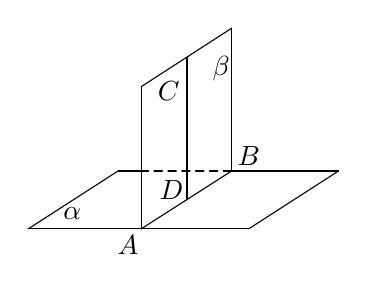
\begin{tikzpicture}[line cap=round,line join=round,scale=0.7]
        \draw (0,0)-- (1.63,1.05);
        \draw (5.63,1.05)-- (4,0);
        \draw (2.05,2.58)-- (3.69,3.64);
        \draw (0,0)-- (4,0);
        \draw (2.05,2.58)-- (2.05,0);
        \draw (2.05,0)-- (3.69,1.05);
        \draw (3.69,1.05)-- (3.69,3.64);
        \draw (2.88,3.11)-- (2.88,0.53);
        \draw (1.63,1.05)-- (2.05,1.05);
        \draw [densely dashed] (3.69,1.05)-- (2.05,1.05);
        \draw (3.69,1.05)-- (5.63,1.05);


        \draw (0.8,0) node[above] {$\alpha$};
        \draw (3.5,2.9) node {$\beta$};
        \draw (2.55,2.5) node {$C$};
        \draw (1.810256579999996,-0.3) node {$A$};
        \draw (4,1.32) node {$B$};
        \draw (2.6,0.7) node {$D$};
      \end{tikzpicture}
      \caption{}\label{fig-190703-1940}
    \end{minipage}
    \end{figure}


\lianxi
\begin{exercise}
    若平面 $\alpha \perp$ 平面 $\gamma$, 平面 $\beta\perp$ 平面 $\gamma$, 判断 $\alpha$ 与 $\beta$ 的位置关系.
\end{exercise}
\beginsolution
    相交或平行 (面面垂直没有传递性).
\endsolution

\begin{exercise}
    若平面 $\alpha\perp$ 平面 $\beta$, 直线 $l\perp$ 平面 $\beta$, 判断 $l$ 与 $\alpha$ 的位置关系.
\end{exercise}
\beginsolution
    若 $l$ 与 $\alpha$ 相交, 则 $l\subset \alpha$; 若 $l$ 与 $\alpha$ 不相交, 则 $l\parallel \alpha$.
\endsolution

\begin{exercise}
    如图 \ref{fig-211107-2000} 所示, 在正方体 $ABCD\text{--}A_1 B_1 C_1 D_1$ 中, 判断平面 $AB_1 C$ 与平面 $BDD_1 B_1$ 的位置关系.
\end{exercise}
\beginsolution
    连接 $BD_1$, 可证 $BD_1\perp$ 平面 $ACB_1$ (见上一节课后练习 4), 所以平面 $AB_1 C\perp$ 平面 $BDD_1 B_1$.
\endsolution

\begin{figure}[htb]
    \small\centering
    \begin{minipage}[b]{0.45\linewidth}
        \centering
        \includegraphics[scale=1.3]{2021-1107-2000-crop}
        \caption{}\label{fig-211107-2000}
    \end{minipage}
    \hskip 0.5cm
    \begin{minipage}[b]{0.45\linewidth}
        \centering
        \includegraphics[scale=1.3]{2021-1107-2010-crop}
        \caption{}\label{fig-211107-2010}
    \end{minipage}
\end{figure}

\begin{exercise}
    如图 \ref{fig-211107-2010} 所示, 在正方体 $ABCD\text{--}A_1 B_1 C_1 D_1$ 中, $E$ 为 $BB_1$ 中点, 求二面角 $E\text{--}AC\text{--}D_1$ 的大小.
\end{exercise}
\beginsolution
    方法一: 连接 $B_1D$, 由上一节课后练习 4 知, $B_1D\perp$ 平面 $ACD_1$. 连接 $BD$, 设其与 $AC$ 交于点 $F$, 则在正方形 $ABCD$ 中, $F$ 为 $BD$ 中点, 连接 $EF$. 因为 $E$ 为 $BB_1$ 中点, 所以 $EF\parallel B_1D$, 则 $EF\perp$ 平面 $ACD$, 从而平面 $AEC\perp$ 平面 $AD_1C$, 即二面角 $E\text{--}AC\text{--}D_1$ 的大小为 $90^\circ$. 

    方法二: 连接 $BD$, 设其与 $AC$ 交于点 $F$, 则在正方形 $ABCD$ 中, $F$ 为 $AC$,$BD$ 的中点. 设题中正方体的边长为 $a$, 则
    \[AD_1=CD_1= \sqrt2a,\quad BE=\frac{a}2,\quad
        EC=EA= \frac{\sqrt5}2 a,\]
    所以 $EF\perp AC$, $D_1F\perp AC$, 
    \mymarginpar{也可以用 $\mathrm{Rt}\triangle BEF\sim \mathrm{Rt}\triangle DD_1F$ 证明 $\angle EFD= 90^\circ$ (矩形 $BDD_1B_1$ 的邻边比为 $1: \sqrt2$).}
    即 $\angle EFD_1$ 为二面角 $E\text{--}AC\text{--}D_1$ 的平面角. 连接 $B_1D_1$, $ED_1$, 则在矩形 $BDD_1B_1$ 中, 
    \[BF= DF= \frac{\sqrt2}2 a,\quad 
        EF= \frac{\sqrt3}2 a,\quad
        D_1F= \frac{\sqrt6}2 a,\quad
        D_1E= \frac32 a,\]
    即 $D_1E^2= EF^2+ D_1F^2$, 表明 $\angle EFD_1= 90^\circ$, 所以二面角 $E\text{--}AC\text{--}D_1$ 的大小为 $90^\circ$.
\endsolution
    
\subsection{要点导学\quad 各个击破}
\subsubsection{面面垂直的判定}
\begin{example}
    如图 \ref{fig-190704-1830} 所示, 在四棱锥 $P\text{--}ABCD$ 中, $AB\parallel CD$, $AB\perp AD$, $CD=2AB$, 平面 $PAD\perp$ 底面 $ABCD$, $E$ 和 $F$ 分别为 $CD$ 和 $PC$ 的中点. 求证: 平面 $BEF\perp$ 平面 $PCD$.
\end{example}
\beginsolution
    因为 $AB\parallel CD$, $CD=2AB$, $E$ 为 $CD$ 的中点, 所以 $DE\parallel AB$, $DE=AB$, 则四边形 $ABED$ 为平行四边形. 由 $AB\perp CD$ 知, 四边形 $ABED$ 为矩形, $CD\perp BE$, $CD\perp AD$. 因为平面 $PAD\perp$ 底面 $ABCD$, 所以 $CD\perp$ 平面 $PAD$, 则 $CD\perp PD$. 因为 $E$ 和 $F$ 分别为 $CD$ 和 $PC$ 的中点, 所以 $EF\parallel PD$, 则 $CD\perp EF$. 结合 $CD\perp BE$ 知 $CD\perp$ 平面 $BEF$, 故平面 $BEF\perp$ 平面 $PCD$.
\endsolution

    \begin{figure}[htb]
    \small
    \centering
    \begin{minipage}[b]{0.45\linewidth}
      \centering
      \begin{tikzpicture}[line cap=round,line join=round,scale=1.4]        
      \draw (0,0,0) coordinate (A) +(0,0.1,0) node[left] {$A$}
            (0,0,1) coordinate (B) node[left] {$B$}
            (2,0,2) coordinate (C) +(0.1,0,0) node[right] {$C$}
            (2,0,0) coordinate (D) node[right] {$D$}
            (0,1.4,0) coordinate (P) node[left] {$P$}
            ($(C)!0.5!(D)$) coordinate (E) +(0.1,0,0) node[right] {$E$}
            ($(C)!0.5!(P)$) coordinate (F) node[anchor=south west] {$F$};
      
      \draw (P)--(B)--(C)--(D)--(P)--(C) (B)--(F)--(E);
      \draw[densely dashed] (P)--(A) (D)--(A)--(B)--(E); 
      \end{tikzpicture}
      \caption{}\label{fig-190704-1830}
    \end{minipage}
    \hskip 0.5cm  
    \begin{minipage}[b]{0.45\linewidth}
      \centering
      \begin{tikzpicture}[line cap=round,line join=round,scale=1.3]
      \draw (0.1,0,2) coordinate (A) node[right] {$A$}
            (0,0,0) coordinate (B) node[right] {$B$}
            (0,1.732,1) coordinate (C) node[right] {$C$}
            (-1.9,0,2) coordinate (A1) node[left] {$A_1$}
            (-2,0,0) coordinate (B1) node[left] {$B_1$}
            (-2,1.732,1) coordinate (C1) node[left] {$C_1$}
            ($(A)!0.5!(B)$) coordinate (D) node[right] {$D$}
            ($(C)!0.5!(B)$) coordinate (E) node[right] {$E$}
            ($(C1)!0.5!(A1)$) coordinate (F) node[left] {$F$};
      
      \draw (A1)--(C1)--(C)--(A1)--(A)--(C)--(B)--(A) (C)--(D);
      \draw[densely dashed] (D)--(A1)--(B1)--(B) (B1)--(C1) (E)--(F); 
      \end{tikzpicture}
      \caption{}\label{fig-190704-1840}
    \end{minipage}
    \end{figure}
    
\lianxi
\begin{exercise}[s]
    如图 \ref{fig-190704-1840} 所示, 在三棱柱 $ABC\text{--}A_1B_1C_1$ 中, 侧棱 $A_1A\perp$ 底面 $ABC$, $AC=BC$, $D$, $E$, $F$ 分别为棱 $AB$, $BC$, $A_1 C_1$ 的中点. 
    
    (1) 求证: $EF\parallel$ 平面 $ABB_1A_1$;
    
    (2) 求证: 平面 $A_1 CD\perp$ 平面 $ABB_1A_1$.
\end{exercise}
\beginsolution
    (1) 连接 $DE$, 则
    \[DE\parallel AC\parallel A_1F,\quad
        DE= \frac12 AC= A_1F,\]
    所以四边形 $DEFA_1$ 为平行四边形, $EF\parallel A_1D$, 从而 $EF\parallel$ 平面 $ABB_1A_1$.

    (2) 因为 $A_1A\perp$ 底面 $ABC$, 所以 $A_1A\perp CD$. 由 $AC= BC$ 知, $CD\perp AB$, 则 $CD\perp$ 平面 $ABB_1A_1$, 故 平面 $A_1 CD\perp$ 平面 $ABB_1A_1$.
\endsolution
    
\subsubsection{面面垂直的性质}
\begin{example}
    如图 \ref{fig-190704-1850} 所示, 在三棱锥 $S\text{--}ABC$ 中, 平面 $SAB\perp$ 平面 $SBC$, $AB\perp BC$, $AS=AB$. 过 $A$ 点作 $AF\perp SB$, 垂足为 $F$, 而 $E$,$G$ 分别为棱 $SA$,$SC$ 的中点.
    
    (1) 求证: 平面 $EFG\parallel$ 平面 $ABC$;\qquad
    (2) 求证: $BC\perp SA$.
\end{example}
\beginsolution
    (1) 因为 $E$,$G$ 分别为棱 $SA$,$SC$ 的中点, 所以 $EG\parallel AC$. 由 $AS=AB$ , $AF\perp SB$ 知, $F$ 为 $SB$ 中点, 则 $EF\parallel AB$, 所以平面 $EFG\parallel$ 平面 $ABC$.

    (2) 因为平面 $SAB\perp$ 平面 $SBC$, $AF\perp SB$, 所以 $AF\perp$ 平面 $SBC$, 则 $AF\perp BC$. 结合 $AB\perp BC$ 知 $BC\perp$ 平面 $SAB$, 故 $BC\perp SA$.
\endsolution

    \begin{figure}[htb]
    \small
    \centering
    \begin{minipage}[b]{0.45\linewidth}
      \centering
      \begin{tikzpicture}[line cap=round,line join=round,scale=0.9]        
      \draw (0,0,0) coordinate (A) node[left] {$A$}
            (2,0,2) coordinate (B) node[below] {$B$}
            (4,0,0) coordinate (C) node[right] {$C$}
            (1,2.449,1) coordinate (S) node[above] {$S$}
            ($(A)!0.5!(S)$) coordinate (E) node[left] {$E$}
            ($(B)!0.5!(S)$) coordinate (F) node[anchor=north west] {$F$}
            ($(C)!0.5!(S)$) coordinate (G) node[anchor=south west] {$G$};
      
      \draw (A)--(B)--(C)--(S)--(A)--(F)--(G) (S)--(B) (E)--(F);
      \draw[densely dashed] (C)--(A) (E)--(G); 
      \end{tikzpicture}
      \caption{}\label{fig-190704-1850}
    \end{minipage}
    \hskip 0.5cm  
    \begin{minipage}[b]{0.45\linewidth}
      \centering
      \begin{tikzpicture}[line cap=round,line join=round,scale=1.5]
      \draw (0,0,0) coordinate (O) node[below] {$O$}
            ({sin(166)},0,{cos(166)}) coordinate (A) +(0.05,0,0) node[anchor=south west] {$A$}
            (1,0,0) coordinate (B) node[below] {$B$}
            (-1,0,0) coordinate (C) node[below] {$C$}
            (C)++(0,1.5,0) coordinate (D) node[left] {$D$}
            ($(D)+0.5*(A)-0.5*(C)$) coordinate (E) node[right] {$E$}
            ({sin(218)},0,{cos(218)}) coordinate (F) +(-0.05,0.05,0) node[left] {$F$};
      
      \draw[smooth,domain=90:153,variable=\t] plot({sin(\t)},0,{cos(\t)});
      \draw[densely dashed,smooth,domain=153:270,variable=\t] plot({sin(\t)},0,{cos(\t)});
      
      \draw (O)--(D)--(C)--(B)--(D)--(E)--(B);
      \draw[densely dashed] (O)--(F)--(D) (C)--(A)--(E) (A)--(B); 
      \end{tikzpicture}
      \caption{}\label{fig-190704-1900}
    \end{minipage}
    \end{figure}
    
\lianxi
\begin{exercise}[s]
    如图 \ref{fig-190704-1900} 所示, 已知 $BC$ 是半径为 1 的半圆 $O$ 的直径, $A$ 是半圆周上不同于 $B$, $C$ 的点, $F$ 为弧 $AC$ 的中点. 在梯形 $ACDE$ 中, $DE\parallel AC$, 且 $AC=2DE$, 平面 $ACDE\perp$ 平面 $ABC$.
    
    (1) 求证: 平面 $ABE\perp$ 平面 $ACDE$;
    
    (2) 求证: 平面 $OFD\parallel $ 平面 $BAE$.
\end{exercise}
\beginsolution
    (1) 因为 $BC$ 为直径, 所以 $AB\perp AC$. 由平面 $ACDE\perp$ 平面 $ABC$ 知 $AB\perp$ 平面 $ACDE$, 则平面 $ABE\perp$ 平面 $ACDE$.

    (2) 设 $AC$ 与 $OF$ 交于点 $G$, 连接 $DG$. 因为 $F$ 为弧 $AC$ 的中点, 所以 $G$ 为 $AC$ 的中点. 由 $AC=2DE$ 知 
    \[AG= \frac12 AC= DE.\]
    而 $DE\parallel AC$, 即 $DE\parallel AG$, 所以四边形 $ACDE$ 为平行四边形, $DE\parallel AE$, 因此平面 $OFD\parallel $ 平面 $BAE$.
\endsolution
    
\subsubsection{面面垂直的探索性问题}
\begin{example}
    如图 \ref{fig-190704-1920} 所示, 在三棱锥 $P\text{--}ABC$ 中, $AB=AC$, $D$ 为 $BC$ 的中点, $PO\perp$ 平面 $ABC$, 垂足 $O$ 落在线段 $AD$ 上. 已知 $BC=8$, $PO=4$, $AO=3$, $OD=2$.
    
    (1) 求证: $AP\perp BC$.
    
    (2) 线段 $AP$ 上是否存在点 $M$, 使得二面角 $A\text{--}MC\text{--}B$ 为直二面角\,?
\end{example}
\beginsolution
    (1) 因为 $AB=AC$, $D$ 为 $BC$ 的中点, 所以 $AD\perp BC$. 又因为 $PO\perp$ 平面 $ABC$, 所以 $PO\perp BC$. 由 $O\in AD$ 知 $BC\perp$ 平面 $PAD$, 则 $AP\perp BC$.

    (2) 存在符合题意的点 $M$, 理由如下:

    \mymarginpar{(2) 中也可用空间向量求解, 并以 $O$ 为原点建立空间直角坐标系, 此时转为说明平面 $PAC$ 的法向量可由平面 $BMC$ 中的两个不共线的向量 (如 $\overrightarrow{BC}$,$\overrightarrow{BM}$) 线性组合表示. 不建议计算平面 $BMC$ 的法向量, 因为点 $M$ 的位置还没有确定.}
    由题意, 三棱锥 $P\text{--}ABC$ 关于平面 $PAD$ 对称, 所以若 $BM\perp AP$, 则 $CM\perp AP$, 从而 $AP\perp$ 平面 $BMC$, 平面 $AMC\perp$ 平面 $BMC$, 即二面角 $A\text{--}MC\text{--}B$ 为直二面角. 由已知可得, 
    \[AP=5,\quad AB=\sqrt{41},\quad
        PD= 2\sqrt5,\quad PB=6,\]
    所以 $\triangle ABP$ 为锐角三角形, 即当 $BM\perp AP$ 时, 垂足 $M$ 在线段 $AP$ 上, 符合题意.
\endsolution

    \begin{figure}[htb]
    \small
    \centering
    \begin{minipage}[b]{0.45\linewidth}
      \centering
      \begin{tikzpicture}[line cap=round,line join=round,scale=0.5]        
      \draw (0,0,0) coordinate (A) node[left] {$A$}
            (5,0,4) coordinate (B) node[below] {$B$}
            (5,0,-4) coordinate (C) node[right] {$C$}
            (5,0,0) coordinate (D) node[right] {$D$}
            (3,0,0) coordinate (O) node[anchor=north east] {$O$}
            (O)++(0,4,0) coordinate (P) node[left] {$P$}
            ($(A)!0.6!(P)$) coordinate (M) node[left] {$M$};
      
      \draw (M)--(B)--(A)--(P)--(B)--(C)--(P)--(D);
      \draw[densely dashed] (M)--(C)--(A)--(D) (P)--(O); 
      \end{tikzpicture}
      \caption{}\label{fig-190704-1920}
    \end{minipage}
    \hskip 0.5cm  
    \begin{minipage}[b]{0.45\linewidth}
      \centering
      \begin{tikzpicture}[line cap=round,line join=round,scale=1.3]
      \draw (0,0,0) coordinate (A) node[left] {$A$}
            (2,0,0) coordinate (B) node[right] {$B$}
            (1.5,0,0.866) coordinate (C) node[below] {$C$}
            (0,2,0) coordinate (P) node[left] {$P$}
            ($(P)!0.5!(B)$) coordinate (D) node[right] {$D$}
            ($(P)!0.5!(C)$) coordinate (E) node[left] {$E$};
      
      \draw (P)--(A)--(C)--(P)--(B)--(C) (A)--(E)--(D);
      \draw[densely dashed] (D)--(A)--(B); 
      \end{tikzpicture}
      \caption{}\label{fig-190704-1930}
    \end{minipage}
    \end{figure}
    
\lianxi
\begin{exercise}[s]
    如图 \ref{fig-190704-1930} 所示, 在三棱锥 $P\text{--}ABC$ 中, $PA\perp$ 底面 $ABC$, $PA=AB$, $\angle ABC=60^\circ$, $\angle BCA=90^\circ$, 点 $D$, $E$ 分别在棱 $PB$, $PC$ 上, 且 $DE\parallel BC$.
    
    (1) 求证: $BC\perp $ 平面 $PAC$.
    
    (2) 若二面角 $A\text{--}DE\text{--}P$ 为直二面角, 求 $\dfrac{PE}{EC}$ 的值.
\end{exercise}
\beginsolution
    (1) 因为 $PA\perp$ 底面 $ABC$, 所以 $PA\perp BC$. 由 $\angle BCA=90^\circ$ 知 $BC\perp AC_1$, 所以 $BC\perp $ 平面 $PAC$.

    (2) 因为 $DE\parallel BC$, 所以 $DE\perp$ 平面 $PAC$, 则
    \[DE\perp PE,\quad DE\perp AE,\]
    即 $\angle AEP$ 为二面角 $A\text{--}DE\text{--}P$ 的平面角, 结合题意知, $\angle AEP= 90^\circ$. 设 $BC=a$, 则
    \[AB=AP=2a,\quad, AC=\sqrt3a.\]
    \mymarginpar{由解题过程可得, 若 $\mathrm{Rt}\triangle ABC$ 的斜边 $BC$ 上的高为 $AD$, 则
    \[\frac{DB}{DC}= \frac{AB^2}{AC^2}.\]}
    在 $\mathrm{Rt}\triangle PAC$ 中, $PC=\sqrt7a$, 则
    \[\cos APE= \frac2{\sqrt7},\quad
        \cos ACE= \frac{\sqrt3}{\sqrt7}.\]
    而 $PE= PA\cos\angle APE$, $EC= AC\cos\angle ACE$, 故
    \[\frac{PE}{EC}
        = \frac{PA}{AC}\cdot \frac{\cos\angle APE}{\cos\angle ACE}
        = \frac43.\]
\endsolution
    
\subsubsection{课堂评价}

\begin{exercise}
    已知直线 $a$, $b$ 与平面 $\alpha$, $\beta$, $\gamma$, 下列条件中, 能推出 $\alpha \perp\beta$ 的有哪些?
     
    (1) $\alpha \perp\gamma$, $\beta\perp\gamma$;\qquad
    (2) $\alpha \cap\beta=a$, $b\perp a$, $b\subset\beta$;
    
    (3) $a\parallel \beta$, $a\parallel \alpha$;\qquad
    (4) $a\parallel \alpha$, $a\perp\beta$.
\end{exercise}
\beginsolution
    仅 (4) 可行.
\endsolution

\begin{exercise}
    如图 \ref{fig-190705-1820} 所示, 四棱锥 $P\text{--}ABCD$ 的底面为矩形, $AB=\sqrt2$, $BC=1$, $E$ 是 $AB$ 的中点, $DE\perp PA$. 求证: 平面 $PAC\perp$ 平面 $PDE$.
\end{exercise}
\beginsolution
    在矩形 $ABCD$ 中, 可证 $AC\perp DE$, 而 $DE\perp PA$, 所以 $DE\perp$ 平面 $PAC$, 所以平面 $PAC\perp$ 平面 $PDE$.
\endsolution

    \begin{figure}[htb]
    \small
    \centering
    \begin{minipage}[b]{0.45\linewidth}
      \centering
      \begin{tikzpicture}[line cap=round,line join=round,scale=1.6]        
      \draw (0,0,0) coordinate (D) node[anchor=south west] {$D$}
            (0,0,1) coordinate (A) node[below] {$A$}
            (1.414,0,0) coordinate (C) node[right] {$C$}
            (A)++(C) coordinate (B) node[below] {$B$}
            ($0.5*(B)+(0,1.5,0)$) coordinate (P) node[above] {$P$}
            ($(A)!0.5!(B)$) coordinate (E) node[below] {$E$};
      
      \draw (E)--(P)--(A)--(B)--(C)--(P)--(B);
      \draw[densely dashed] (P)--(D)--(A)--(C)--(D)--(E); 
      \end{tikzpicture}
      \caption{}\label{fig-190705-1820}
    \end{minipage}
    \hskip 0.5cm  
    \begin{minipage}[b]{0.45\linewidth}
      \centering
      \begin{tikzpicture}[line cap=round,line join=round,scale=1.4]
      \draw[fill=black] (0,0,0) coordinate (O) node[left] {$O$} circle(0.5pt)
            (-1,0,0) coordinate (A) node[left] {$A$}
            ($(O)-(A)$) coordinate (C) node[right] {$C$}
            ({sin(30)},0,{cos(30)}) coordinate (B) node[below] {$B$}
            ($(O)-(B)$) coordinate (D) +(0,0.1,0) node[left] {$D$}
            (O)++(0,1.2,0) coordinate (A1) node[left] {$A_1$}
            ($(A1)+(B)-(A)$) coordinate (B1) +(0.1,0,0) node[below] {$B_1$}
            ($(A1)+(C)-(A)$) coordinate (C1) node[right] {$C_1$}
            ($(A1)+(D)-(A)$) coordinate (D1) node[above] {$D_1$}
            ($(A1)+(O)-(A)$) coordinate (O1) node[right] {$O_1$};
      
      \draw (A1)--(A)--(B)--(B1)--(A1)--(D1)--(B1)--(C1)--(D1) (B)--(C)--(C1);
      \draw[densely dashed] (D1)--(D)--(A) (D)--(O1)--(C)--(D) (A1)--(O); 
      \end{tikzpicture}
      \caption{}\label{fig-190705-1830}
    \end{minipage}
    \end{figure}
     
\begin{exercise}
    如图 \ref{fig-190705-1830} 所示, 平行六面体 $ABCD\text{--}A_1 B_1 C_1 D_1$ 的底面为正方形, $O_1$, $O$ 分别为上, 下底面的中心, 且点 $A_1$ 在底面 $ABCD$ 上的射影是 $O$. 求证: 平面 $O_1 DC\perp $ 平面 $ABCD$.
\end{exercise}
\beginsolution
    连接 $AC$, $A_1C_1$, 则点 $O$ 和 $O_1$ 分别平分 $AC$ 和 $A_1C_1$,
    \[OC= \frac12 AC= \frac12 A_1C_1= A_1O_1.\]
    因为 $AA_1\parallel CC_1$ 且 $AA_1= CC_1$, 所以四边形  $ACC_1A_1$ 为平行四边形, 则 $OC\parallel A_1O_1$, 从而 四边形 $OCO_1A_1$ 为平行四边形, $A_1O\parallel O_1C$. 而点 $A_1$ 在底面 $ABCD$ 上的射影是点 $O$ 表明 $A_1O\perp$ 平面$ABCD$, 所以 $O_1C\perp$ 平面 $ABCD$, 即 平面 $O_1 DC\perp $ 平面 $ABCD$.
\endsolution

\subsection{课后练习}  
\begin{exercise}
    已知 $PA$ 垂直于正方形 $ABCD$ 所在的平面, 连接 $PB$, $PC$, $PD$, $AC$, $BD$, 判断下列垂直关系是否正确 (填序号):
    
    (1) 平面 $PAB\perp$ 平面 $PBC$;\qquad
    (2) 平面 $PAB\perp$ 平面 $PAD$;
    
    (3) 平面 $PAB\perp$ 平面 $PCD$;\qquad
    (4) 平面 $PAB\perp$ 平面 $PAC$.
\end{exercise}
\beginsolution
    仅 (2) 正确.
\endsolution

\begin{exercise}
    已知 $m$, $n$ 是两条不同的直线, $\alpha$, $\beta$ 是两个不重合的平面, 判断下列命题的真假:
    
    (1) 若 $m\parallel \alpha$, $n\parallel \beta$, $\alpha \parallel \beta$, 则 $m\parallel n$;
    
    (2) 若 $m\parallel \alpha$, $n\parallel \beta$, $\alpha \perp\beta$, 则 $m\perp n$;
    
    (3) 若 $m\perp\alpha$, $n\perp\beta$, $\alpha \perp\beta$, 则 $m\parallel n$;
    
    (4) 若 $m\perp\alpha$, $n\parallel \beta$, $\alpha \parallel \beta$, 则 $m\perp n$.
\end{exercise}
\beginsolution
    (1) 不正确, 线面平行没有传递性;

    (2) 不正确, $m$,$n$ 均可旋转;

    (3) 不正确, 此时 $m\perp n$;

    (4) 正确, 由 $m\perp\alpha$, $\alpha\parallel\beta$ 知 $m\perp\beta$, 而 $n\parallel \beta$, 则 $m\perp n$.
\endsolution

\begin{exercise}
    将边长为 $1$ 的正方形 $ABCD$ 沿对角线 $AC$ 折起后形成三棱锥 $D\text{--}ABC$, 并使二面角 $B\text{--}AC\text{--}D$ 为直二面角, 判断下列命题的真假:
    
    (1) $\triangle DBC$ 是等边三角形; \qquad 
    (2) $AB$ 与 $CD$ 所成的角是 $60^\circ$;
    
    (3) 三棱锥 $D\text{--}ABC$ 的体积是 $\dfrac{\sqrt2}6$;\qquad
    (4) $AC\perp BD$.
\end{exercise}
\beginsolution
    (1) 取 $AC$ 中点 $O$, 连接 $OD$,$OB$. 在原正方形 $ABCD$ 中, $OD\perp AC$, $OB\perp AC$, 则翻折后 $\angle BOD$ 为二面角 $B\text{--}AC\text{--}D$ 的二面角, 由题意 $\angle BOD= 90^\circ$. 因为原正方形 $ABCD$ 的边长为 $1$, 所以
    \[DC=BC=1,\quad OD=OB=\frac{\sqrt2}2,\]
    则 $BD=\sqrt{OB^2+OD^2}=1$, 表明 $\triangle DBC$ 是等边三角形.

    (2) 倍长 $OD$ 至点 $E$, 连接 $EA$,$EC$, 则 $AC$,$DE$ 互相平分, 所以四边形 $AECD$ 为平行四边形, $AE\parallel DC$, 即 $\angle BAE$ 为 $AB$ 与 $CD$ 所成的角. 类似于 (1) 可计算得到 $\triangle ABE$ 为等边三角形. 所以 $\angle BAE= 60^\circ$, 表明 $AB$ 与 $CD$ 所成的角是 $60^\circ$.

    (3) 由 (1), $DO\perp AC$, $DO\perp OB$, 所以 $DO$ 为三棱锥 $O\text{--}ABC$ 的高, 则三棱锥 $D\text{--}ABC$ 的体积为
    \[\frac13 S_{\triangle ABC}\cdot DO
        = \frac13\cdot \frac12\cdot 1^2\cdot \frac{\sqrt2}2
        = \frac{\sqrt2}{12}.\]

    (4) 由 $DO\perp AC$, $BO\perp AC$ 知 $AC\perp$ 平面 $BOD$, 则 $AC\perp BD$.

    综上所述, 仅 (3) 错误.
\endsolution
  
\begin{exercise}
    如图 \ref{fig-190705-1850} 所示, 在三棱锥 $P\text{--}ABC$ 中, $PA=PB$, $\angle ABC=90^\circ$, 平面 $PAB\perp$ 平面 $ABC$, $D$ 和 $E$ 分别是 $AB$ 和 $AC$ 的中点.
    
    (1) 求证: $AB\perp PE$;\qquad
    (2) 求证: $PA\perp BC$.
\end{exercise}
\beginsolution
    (1) 因为 $PA=PB$, $D$ 为 $AB$ 中点, 所以 $PD\perp AB$. 又由 $E$ 为 $AC$ 中点知 $DE\parallel BC$, 而 $\angle ABC= 90^\circ$ 表明 $AB\perp BC$, 则 $AB\perp DE$, 所以 $AB\perp$ 平面 $PDE$, 继而 $AB\perp PE$.

    (2) 因为 $PD\perp AB$, 平面 $PAB\perp$ 平面 $ABC$, 所以 $PD\perp$ 平面 $ABC$, 则 $PD\perp BC$. 结合 $AB\perp BC$ 知, $BC\perp$ 平面 $PAB$, 故 $PA\perp BC$.
\endsolution

    \begin{figure}[htb]
    \small
    \centering
    \begin{minipage}[b]{0.45\linewidth}
      \centering
      \begin{tikzpicture}[line cap=round,line join=round,scale=1.1]
      \draw (0,0,0) coordinate (A) +(0,0.1,0) node[left] {$A$}
            (0,0,2) coordinate (B) node[below] {$B$}
            (B)+(3,0,0) coordinate (C) node[below] {$C$}
            ($(A)!0.5!(B)$) coordinate (D) +(0.05,0.05,0) node[left] {$D$}
            (D)++(0,1.732,0) coordinate (P) node[left] {$P$}
            ($(A)!0.5!(C)$) coordinate (E) +(-0.1,0.15,0) node[right] {$E$};
      
      \draw (P)--(B)--(C)--(P);
      \draw[densely dashed] (P)--(D)--(E)--(P)--(A)--(B) (A)--(C); 
      \end{tikzpicture}
      \caption{}\label{fig-190705-1850}
    \end{minipage}
    \hskip 0.5cm
    \begin{minipage}[b]{0.45\linewidth}
        \centering
        \begin{tikzpicture}[line cap=round,line join=round,scale=1.2]        
        \draw (0,0,0) coordinate (A) node[left] {$A$}
              (2,0,0) coordinate (B) node[below] {$B$}
              (1,0,1.732) coordinate (C) node[below] {$C$}
              (A)++(0,1.8,0) coordinate (A1) node[left] {$A_1$}
              ($(A1)+(B)-(A)$) coordinate (B1) node[right] {$B_1$}
              ($(A1)+(C)-(A)$) coordinate (C1) node[anchor=north west] {$C_1$}
              ($(B1)!0.5!(B)$) coordinate (E) node[right] {$E$}
              ($(A)!0.5!(C)$) coordinate (F) node[left] {$F$};
        
        \draw (C)--(A)--(A1)--(C)--(C1)--(A1)--(B1)--(C1) (B1)--(B)--(C)--(E);
        \draw[densely dashed] (A)--(B)--(F) (E)--(A1); 
        \end{tikzpicture}
        \caption{}\label{fig-190705-1900}
      \end{minipage}
    \end{figure}

\begin{exercise}
    如图 \ref{fig-190705-1900} 所示, 在正三棱柱 $ABC\text{--}A_1 B_1 C_1$ 中, $E$,$F$ 分别为 $BB_1$,$AC$ 的中点.
    
    (1) 求证: $BF\parallel$ 平面 $A_1 EC$;\qquad
    (2) 求证: 平面 $A_1 EC\perp$ 平面 $ACC_1 A_1$.
\end{exercise}
\beginsolution
    (1) 取 $A_1C$ 中点 $G$, 连接 $GE$,$GF$. 因为 $F$ 为 $AC$ 中点, 所以
    \[FG\parallel AA_1\parallel BE,\quad
        FE= \frac12AA_1= \frac12BB-1= BE,\]
    则四边形 $BEGF$ 为平行四边形, $BF\parallel FG$, 所以 $BF\parallel$ 平面 $A_1 EC$.

    (2) 在正三棱锥 $ABC\text{--}A_1B_1C_1$ 中, 
    \mymarginpar{由解题过程知, 此题条件可减弱, 即底面三角形只需满足 $BA=BC$.}
    $\triangle ABC$ 为等边三角形, 由 $F$ 为 $AC$ 中点知 $BF\perp AC$. 而 $AA_1\perp$ 平面 $ADC$, 则 $AA_1\perp BF$, 所以 $BF\perp$ 平面 $ACC_1A_1$. 由 (1) 知, $BF\parallel EG$, 则 $EG\perp$ 平面 $ACC_1A_1$, 故平面 $A_1 EC\perp$ 平面 $ACC_1 A_1$.
\endsolution

\begin{exercise}
    如图 \ref{fig-190705-1910} 所示, 在四棱锥 $P\text{--}ABCD$ 中, $PA$ 垂直于底面, $AC\perp BD$ 于点 $O$.
    
    (1) 求证: 平面 $PBD\perp$ 平面 $PAC$;
    
    (2) 设 $E$ 为线段 $PC$ 上一点, 若 $AC\perp BE$, 求证: $PA\parallel$ 平面 $BED$.
\end{exercise}

    \begin{figure}[htb]
    \small
    \centering
    \begin{tikzpicture}[line cap=round,line join=round,scale=1.3]
      \draw (0,0,0) coordinate (A) node[left] {$A$}
            (1,0,1.5) coordinate (B) node[below] {$B$}
            (2,0,1.5) coordinate (C) node[below] {$C$}
            (2,0,0) coordinate (D) node[right] {$D$}
            (1.3,0,1) coordinate (O) node[above] {$O$}
            (0,1.7,0) coordinate (P) node[left] {$P$}
            ($(P)!0.667!(C)$) coordinate (E) +(-0.1,0.15,0) node[right] {$E$};
      
      \draw (C)--(B)--(A)--(P)--(B)--(E)--(D)--(C)--(P)--(D);
      \draw[densely dashed] (B)--(D)--(A)--(C); 
      \end{tikzpicture}
      \caption{}\label{fig-190705-1910}
    \end{figure}

\beginsolution
    (1) 因为 $PA\perp$ 底面 $ABCD$, 所以 $PA\perp BD$, 而 $AC\perp BD$, 所以 $BD\perp$ 平面 $PAC$, 则平面 $PBD\perp$ 平面 $PAC$.

    (2) 连接 $EO$. 由 $AC\perp BE$, $AC\perp BD$ 知, $AC\perp$ 平面 $BED$, 则 $AC\perp ED$. 因为 $PA\perp$ 底面$ABCD$, 所以 $PA\perp AC$. 在 $\triangle PAC$ 中, $EO$ 和 $PA$ 均与 $AC$ 垂直, 所以 $EO\parallel PA$, 故 $PA\parallel$ 平面 $BED$.
\endsolution
